
\begin{figure}
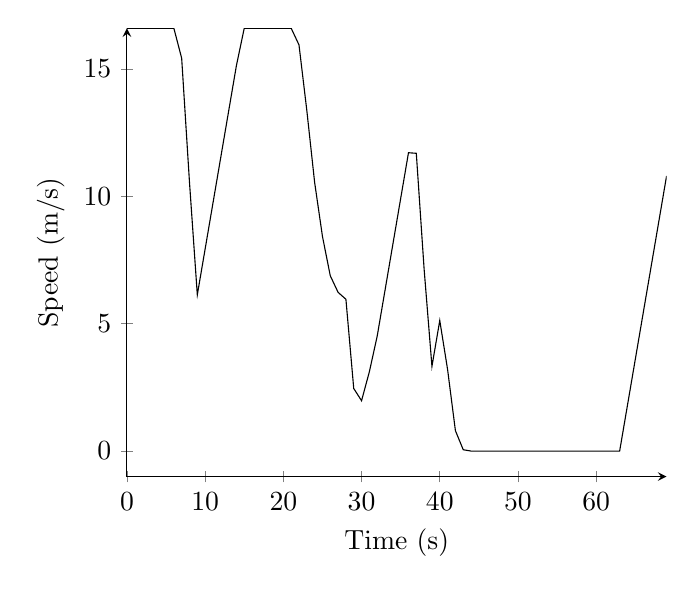
\begin{tikzpicture}
\begin{axis}[
legend style={anchor=west},
axis x line=bottom,
axis y line=left,
ymin=-1,
xlabel=Time (s),
ylabel=Speed (m/s),
]
\addplot[] coordinates {
(0, 16.6)
(1, 16.6)
(2, 16.6)
(3, 16.6)
(4, 16.6)
(5, 16.6)
(6, 16.6)
(7, 15.4214845424)
(8, 10.5475734019)
(9, 6.13471485732)
(10, 7.93471485732)
(11, 9.73471485732)
(12, 11.5347148573)
(13, 13.3347148573)
(14, 15.1347148573)
(15, 16.6)
(16, 16.6)
(17, 16.6)
(18, 16.6)
(19, 16.6)
(20, 16.6)
(21, 16.6)
(22, 15.9465349627)
(23, 13.3755043623)
(24, 10.5483377542)
(25, 8.42935784417)
(26, 6.88262060949)
(27, 6.23165350432)
(28, 5.95933145826)
(29, 2.45657326755)
(30, 1.9771393506)
(31, 3.11641815691)
(32, 4.51247174211)
(33, 6.31247174211)
(34, 8.11247174211)
(35, 9.91247174211)
(36, 11.7124717421)
(37, 11.6895979369)
(38, 7.13950912046)
(39, 3.3259096329)
(40, 5.1259096329)
(41, 3.20167154877)
(42, 0.800786771116)
(43, 0.0532024130037)
(44, 0.0)
(45, 0.0)
(46, 0.0)
(47, 0.0)
(48, 0.0)
(49, 0.0)
(50, 0.0)
(51, 0.0)
(52, 0.0)
(53, 0.0)
(54, 0.0)
(55, 0.0)
(56, 0.0)
(57, 0.0)
(58, 0.0)
(59, 0.0)
(60, 0.0)
(61, 0.0)
(62, 0.0)
(63, 0.0)
(64, 1.8)
(65, 3.6)
(66, 5.4)
(67, 7.2)
(68, 9.0)
(69, 10.8)
};

\end{axis}
\end{tikzpicture}
\label{tik:speed:100:14}
\caption{100 percent diving with GSC on route $14$}
\end{figure}
